\newpage
\section{Durchführung}
\label{sec:Durchführung}
\subsection{Grundlegender Versuchsaufbau}
\label{sec:Aufbau}
Als Sender dient ein gewöhnlicher Lautsprecher, welcher einen Ton mit
konstanter Frequenz
$\nu_0$ liefert. Den Empfänger stellt dementsprechend ein Mikrophon dar.
Um die Relativgeschwindigkeit zwischen Sender um Empfänger zu realisieren wird
ein Wagen auf einer festen Schiene verwendet, welcher über einen Seilzug mit
einem elektrischen Motor (über ein 10-Gang-Getriebe) verbunden ist. Dies
erlaubt relativ präzise definierte, geradlinige Geschwindigkeiten.
Zur Zeitmessung steht eine elektronische Zeitbasis zur Verfügung, welche im
Abstand von $1 \mu \symup{s}$ einen Spannungsimpuls liefert. Ergänzt wird
diese Basis durch ein Zählwerk welches jene Impulse zählen kann sowie einen
dekadischen Untersetzer, welcher den Abstand zwischen zwei Signalen um
$10^2 - 10^7$ erhöht. Zusätzlich stehen zwei Lichtschranken zur Verfügung
sowie eine Logikschaltung um die einzelnen Bestandteile korrekt an zu steuern.

\subsection{Geschwindigkeit des Wagens}
\label{sec:Geschwindigkeit}
Um die Geschwindigkeit des Wagens zu bestimmen, werden zwei Lichtschranken im
Abstand von s $=43\,$cm aufgebaut und an die Schaltung aus Abb.
\ref{fig:Geschwindigkeit-Schaltung} angeschlossen. Dies sorgt dafür,
dass die Zeit zwischen Betätigung der Lichtschranken gemessen wird.
Die Torstufe nimmt also das Signal der ersten Lichtschranken und zählt mit dem Zählwerk
die eingehenden Impulse, die durch den Untersetzer und des Zeitbasisgenerator
generiet werden, aber nur so lange bis das Signal der zweiten Lichtschranke eingeht.
Der Aufbau ergibt sich damit zu dem in Abb. \ref{fig:Geschwindigkeit}
dargestellten.
\begin{figure}
  \centering
  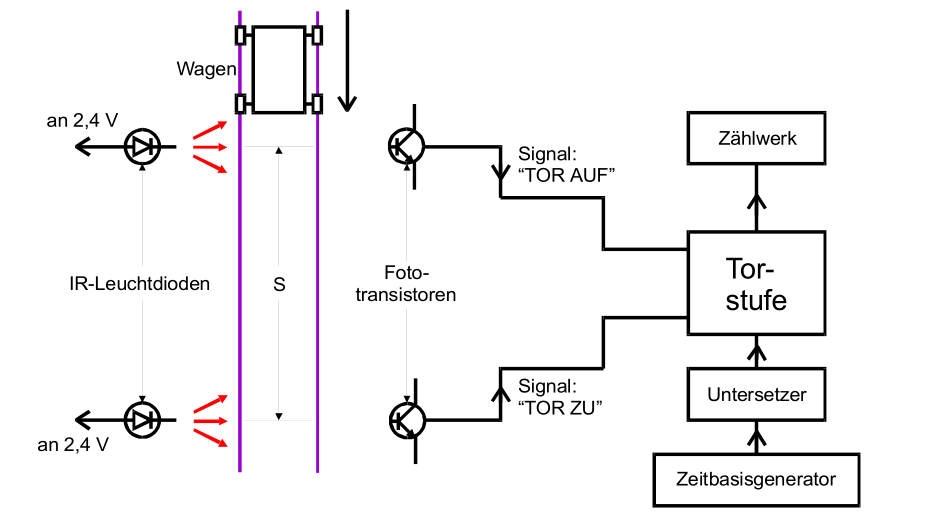
\includegraphics[width = \textwidth]{./Abbildungen/Geschwindigkeit.PNG}
  \caption{Aufbau zur gangabhängigen Geschwindigkeit des Wagens \cite{Anleitung}.}
  \label{fig:Geschwindigkeit}
\end{figure}
\begin{figure}
  \centering
  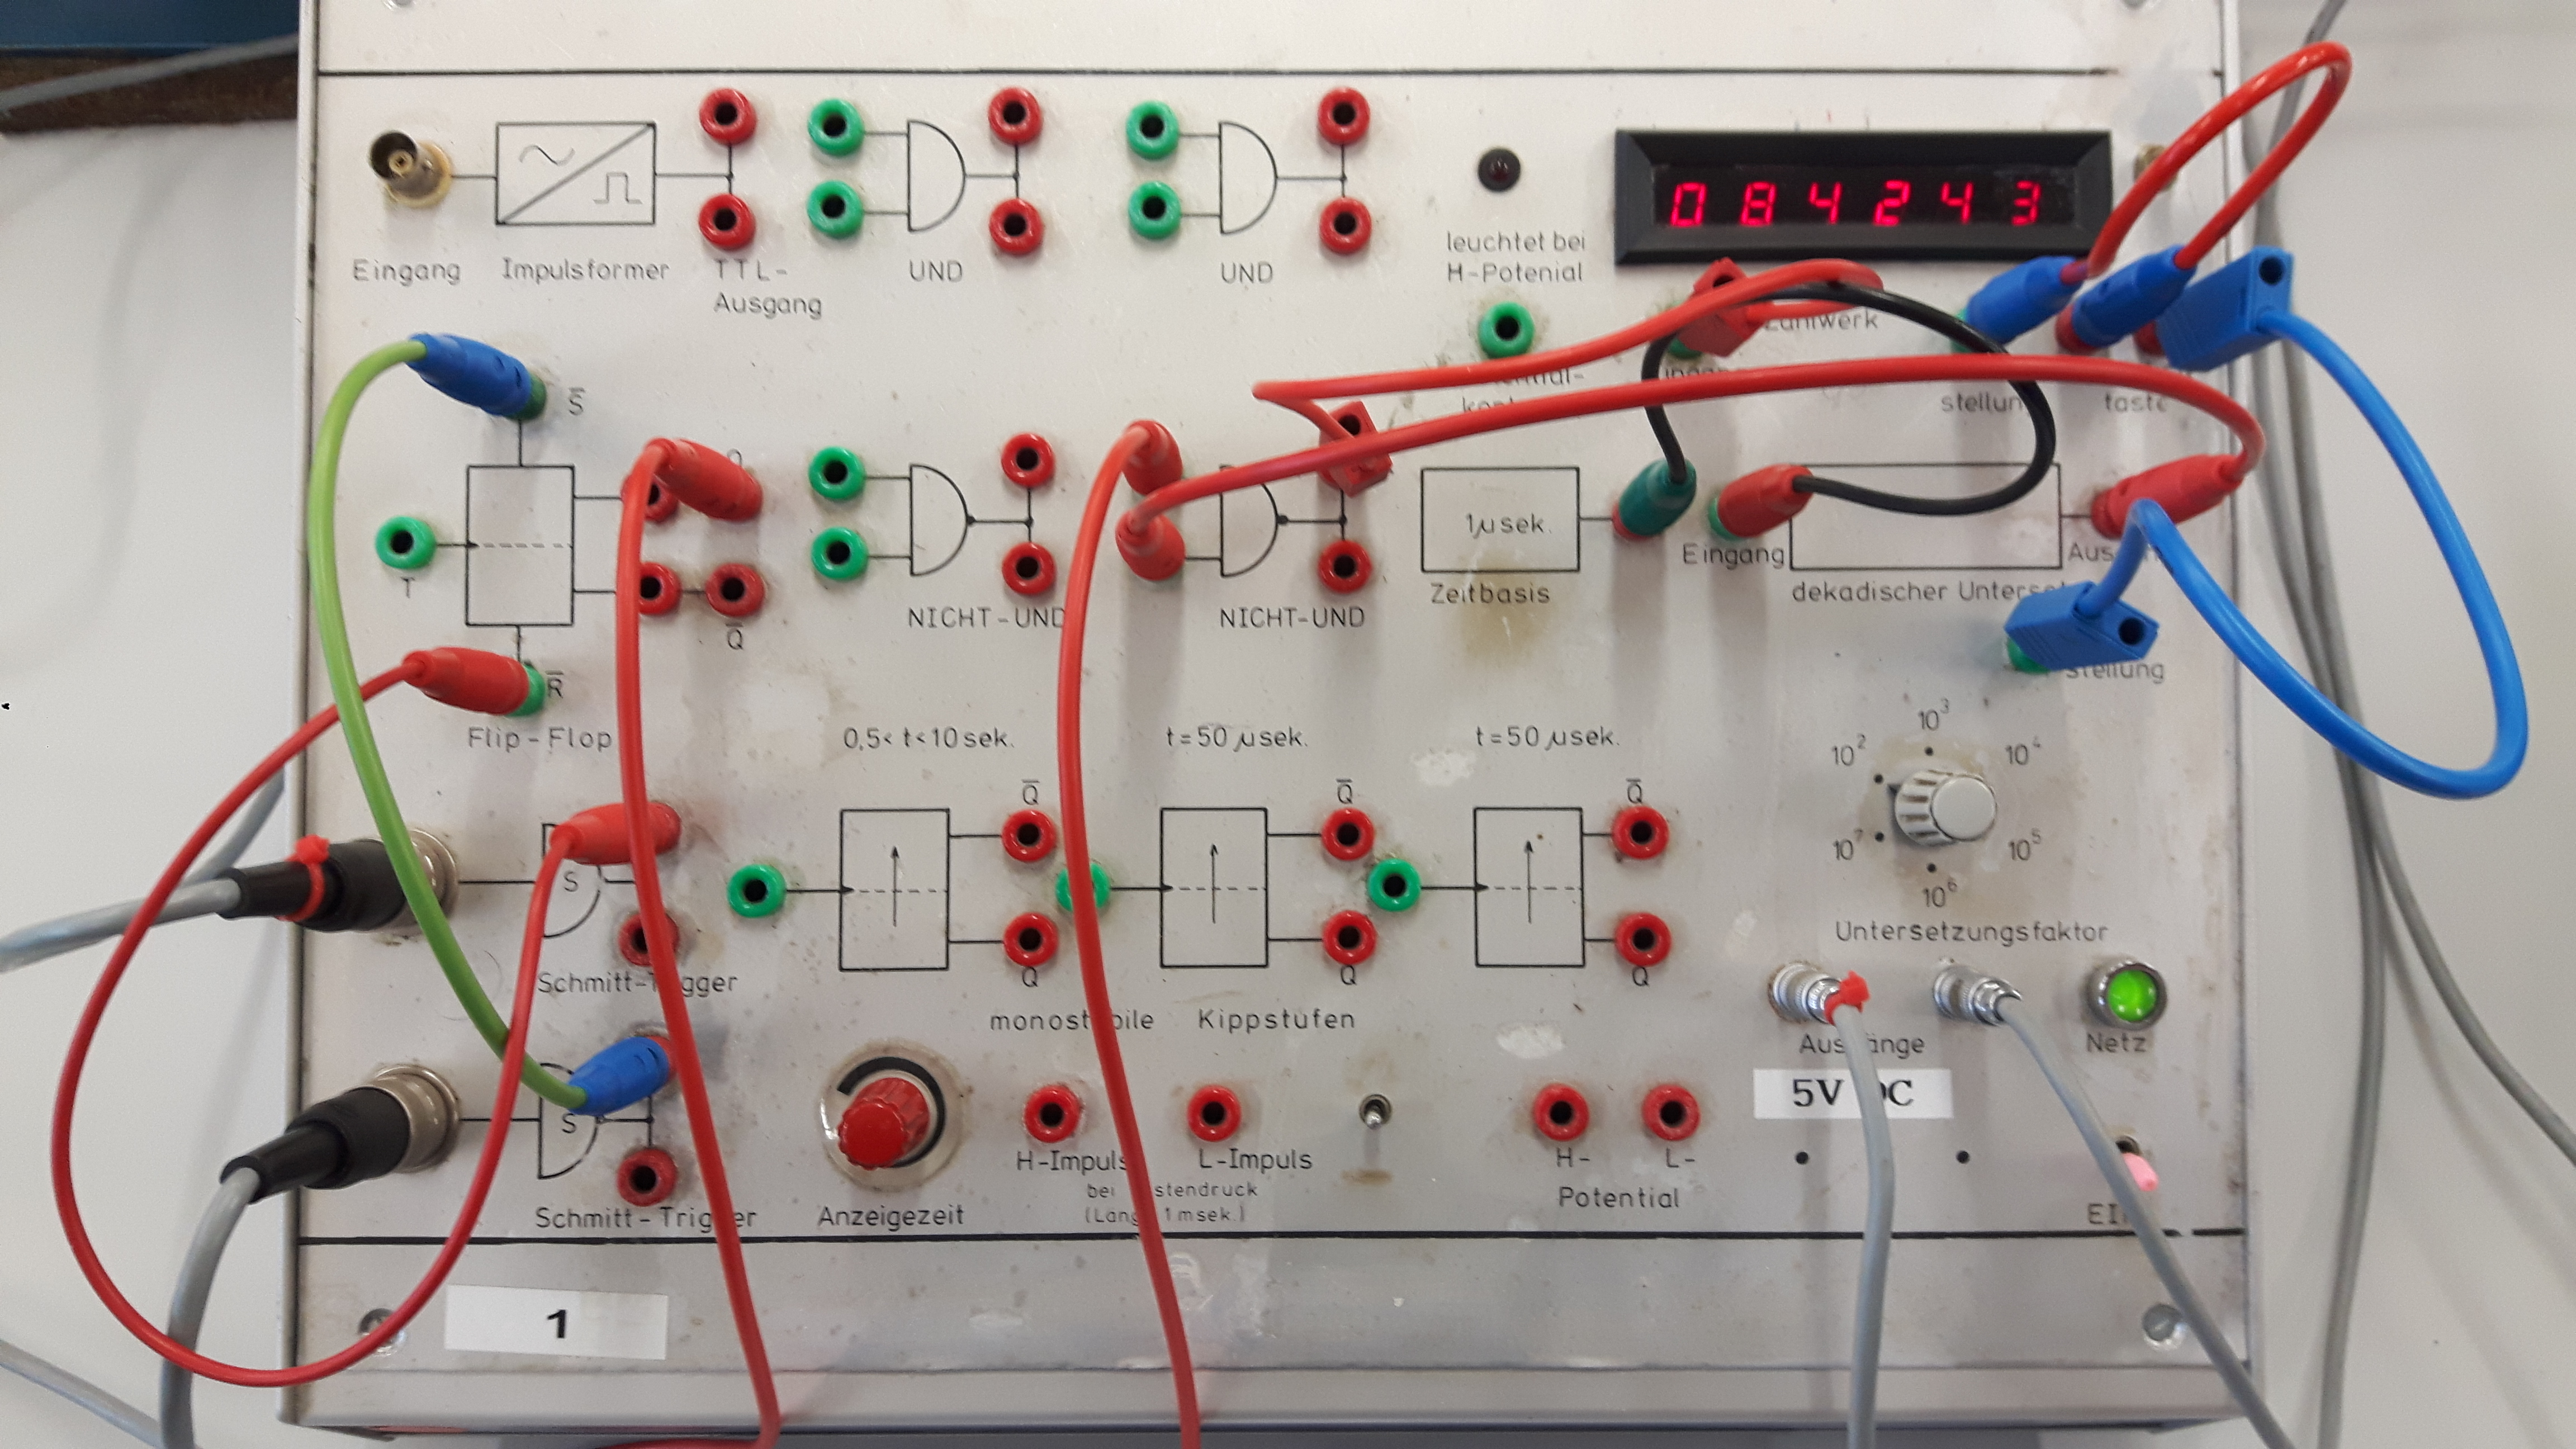
\includegraphics[height = 7cm]{./Abbildungen/Geschwindigkeit-Schaltung.jpg}
  \caption{Verkabelung der Schaltung zur Bestimmung der Geschwindigkeit des Wagens.}
  \label{fig:Geschwindigkeit-Schaltung}
\end{figure}

\subsection{Wellenlänge des Signals}
\label{sec:Wellenlänge}
\begin{figure}
  \centering
  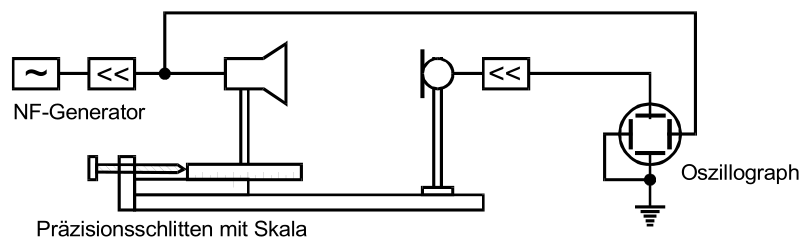
\includegraphics[width = \textwidth]{./Abbildungen/Schallgeschwindigkeit.PNG}
  \caption{Aufbau zur Bestimmung der Wellenlänge des Signals \cite{Anleitung}.}
  \label{fig:Wellenlänge}
\end{figure}

% Mit dem in Abb. \ref{fig:Wellenlänge} dargestellten Aufbau lässt sich die
% Wellenlänge $\lambda_0$ des Signals messen, indem am Oszilloskop das direkt
% abgegriffene Signal, mit dem der Lautsprecher betrieben wird, mit dem über das
% Mikrophon aufgenommenen Signal zu einer Lissajous-Figur überlagert wird.
Die Wellenlänge $\lambda_0$ des Signals lässt sich messen, indem das Signal
des Lautsprechers mit dem selben Signal, nur über ein Mircrophon aufgenommen,
überlagert wird. Das wird durch ein Oszilloskop und Lissajous-Figuren verwirklicht.
Der genau Aufbau ist in Abb. \ref{fig:Wellenlänge} dargestellt.
Anschließend wird der Sender so verschoben, dass beide Signale in Phase
schwingen. Nun kann der Sender verschoben werden, bis die Signale gegenphasig
schwingen. Der Abstand zwischen diesen beiden Punkten entspricht der halben
Wellenlänge.
\FloatBarrier

\subsection{Bestimmung der Frequenz}
\label{sec:Frequenz}

\begin{figure}
  \centering
  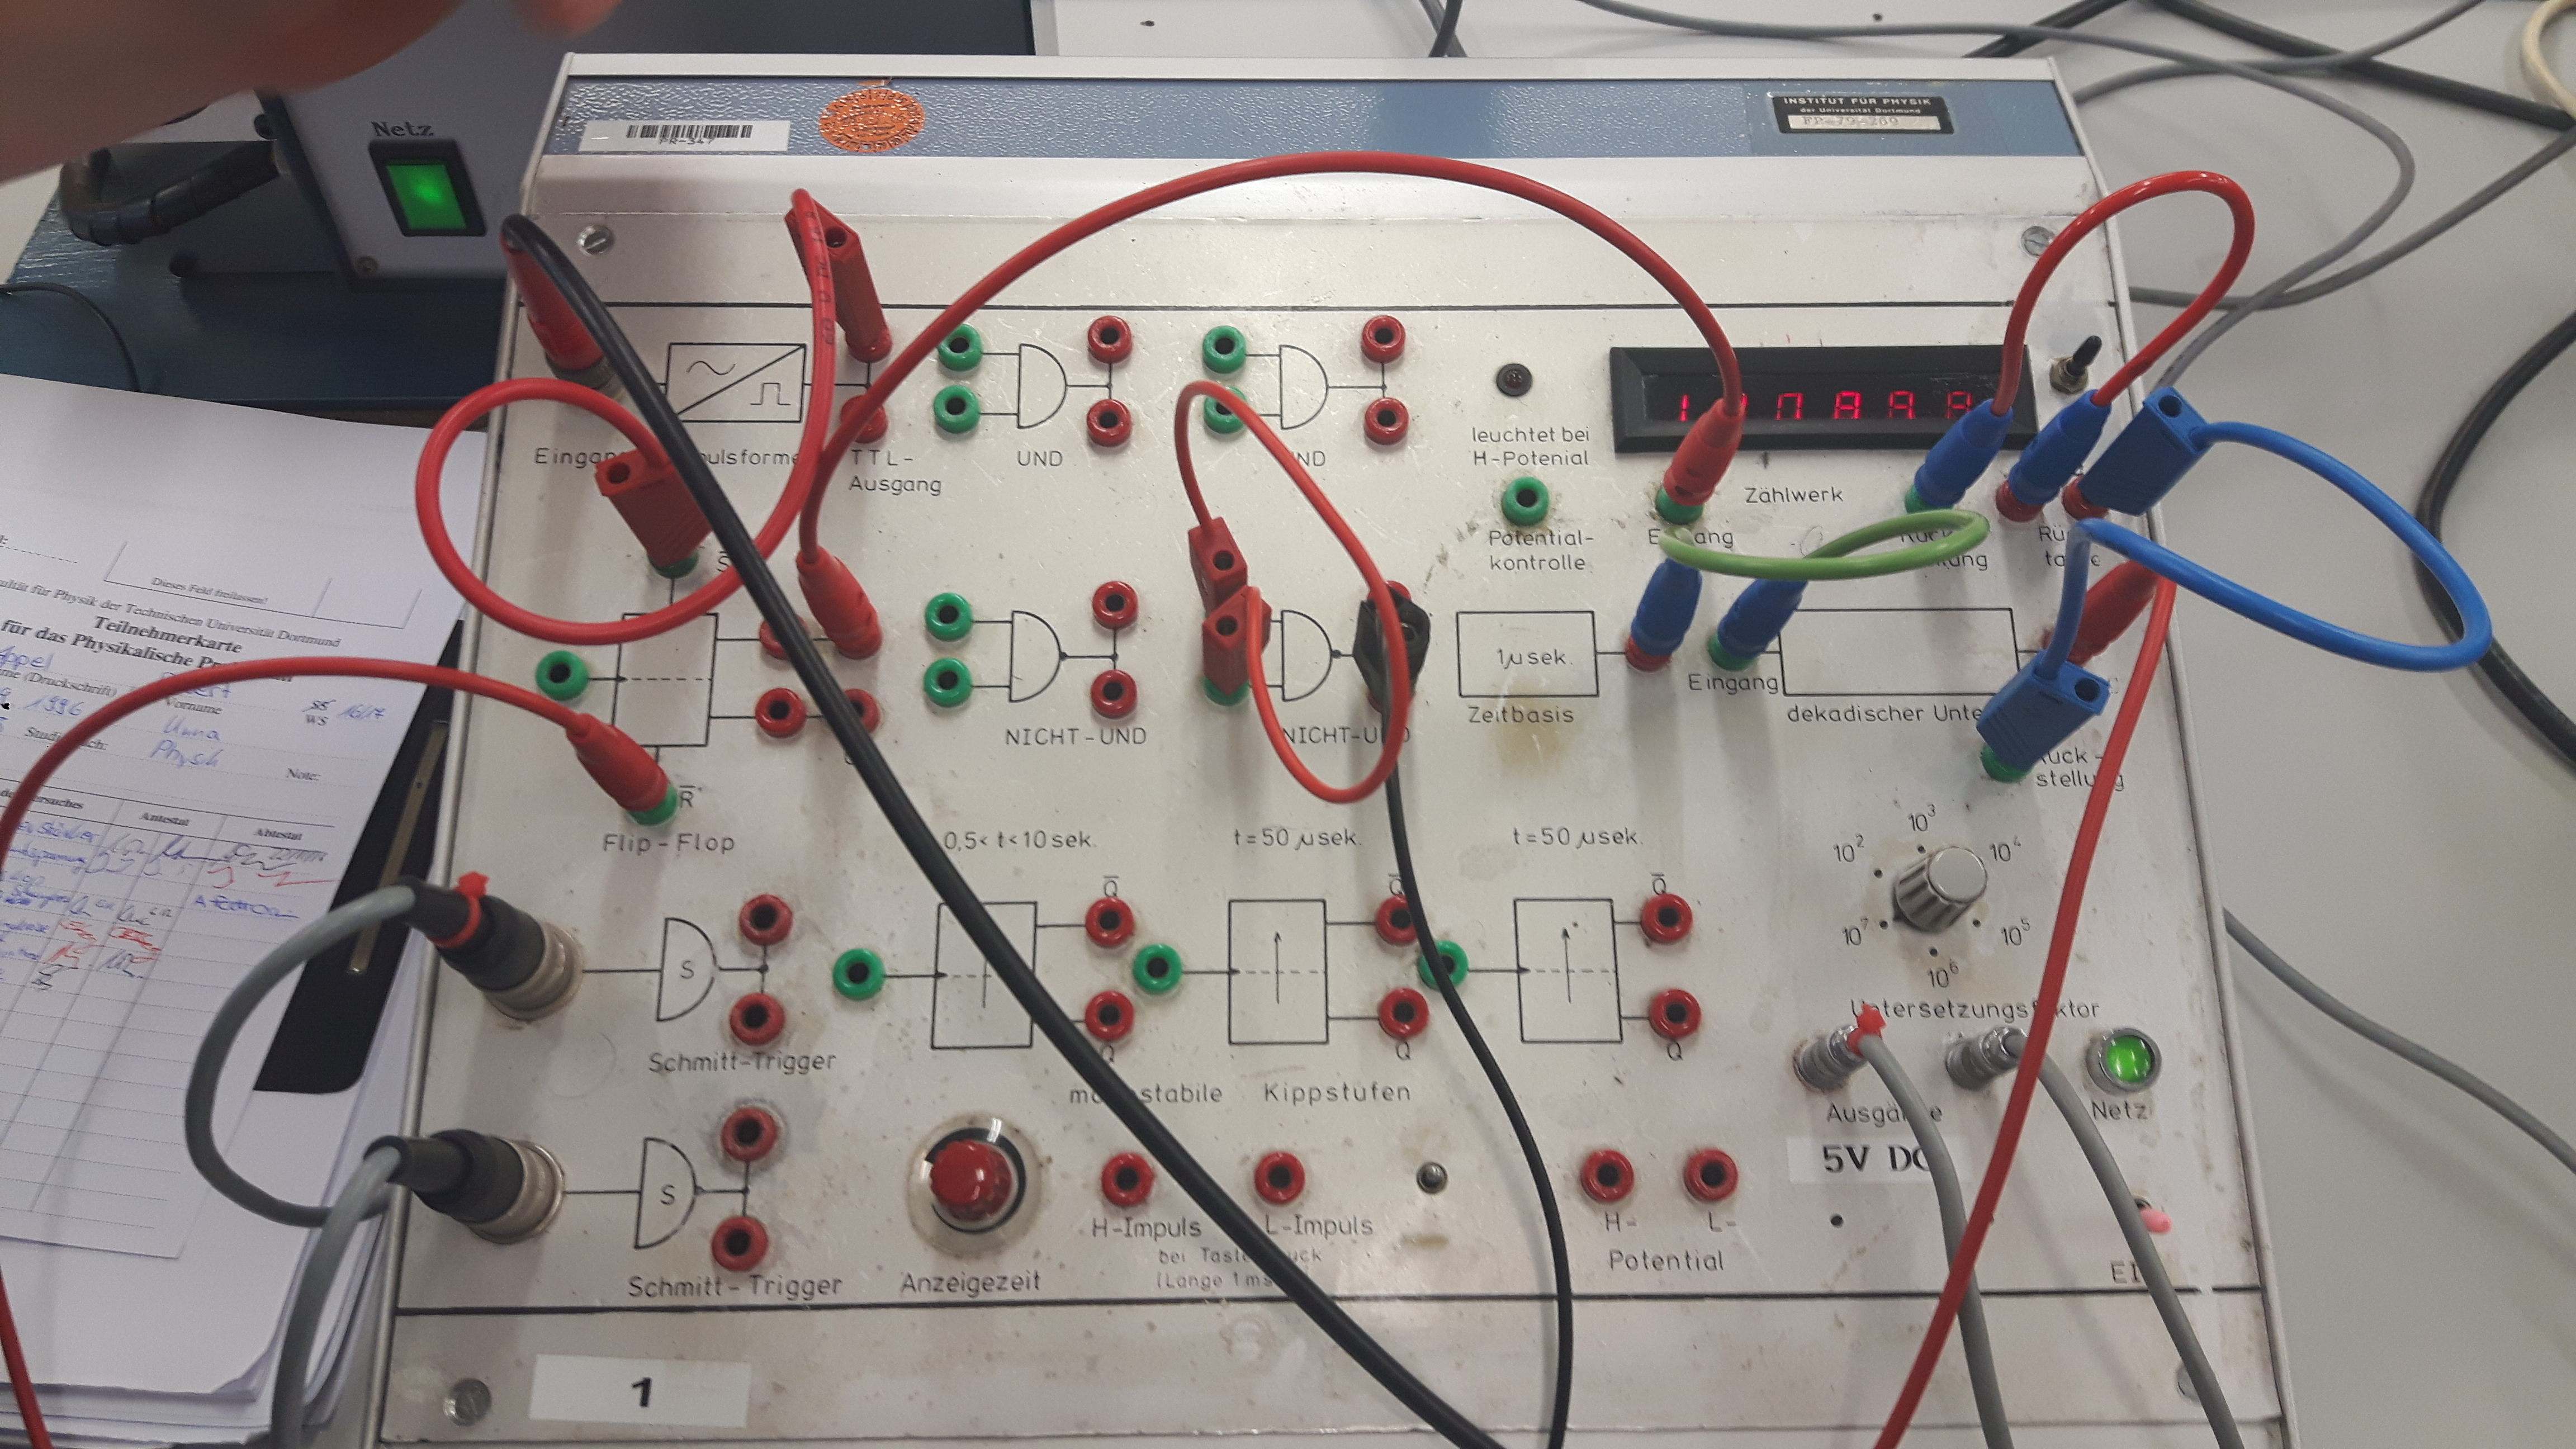
\includegraphics[width = \textwidth]{./Abbildungen/Frequenzmessung.jpg}
  \caption{Schaltung zur Messung der Ruhefrequenz.}
  \label{fig:Ruhefrequenz}
\end{figure}

\begin{figure}
  \centering
  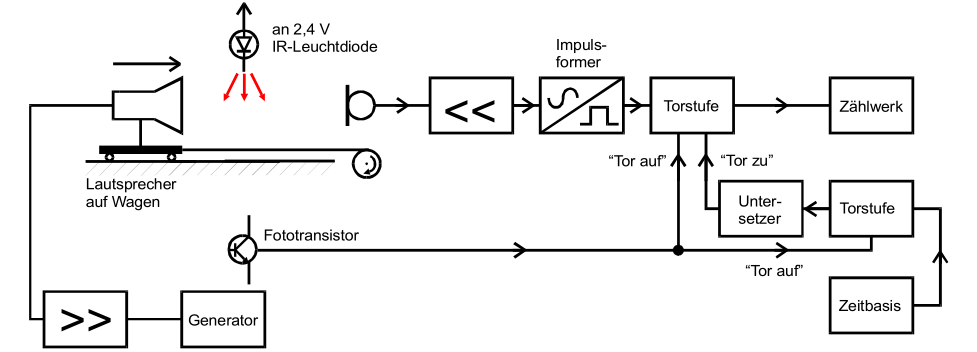
\includegraphics[width = \textwidth]{./Abbildungen/Unbenann.PNG}
  \caption{Aufbau zur Messung der geschwindigkeitsabhängigen Frequenz \cite{Anleitung}.}
  \label{fig:vf}
\end{figure}

\begin{figure}
  \centering
  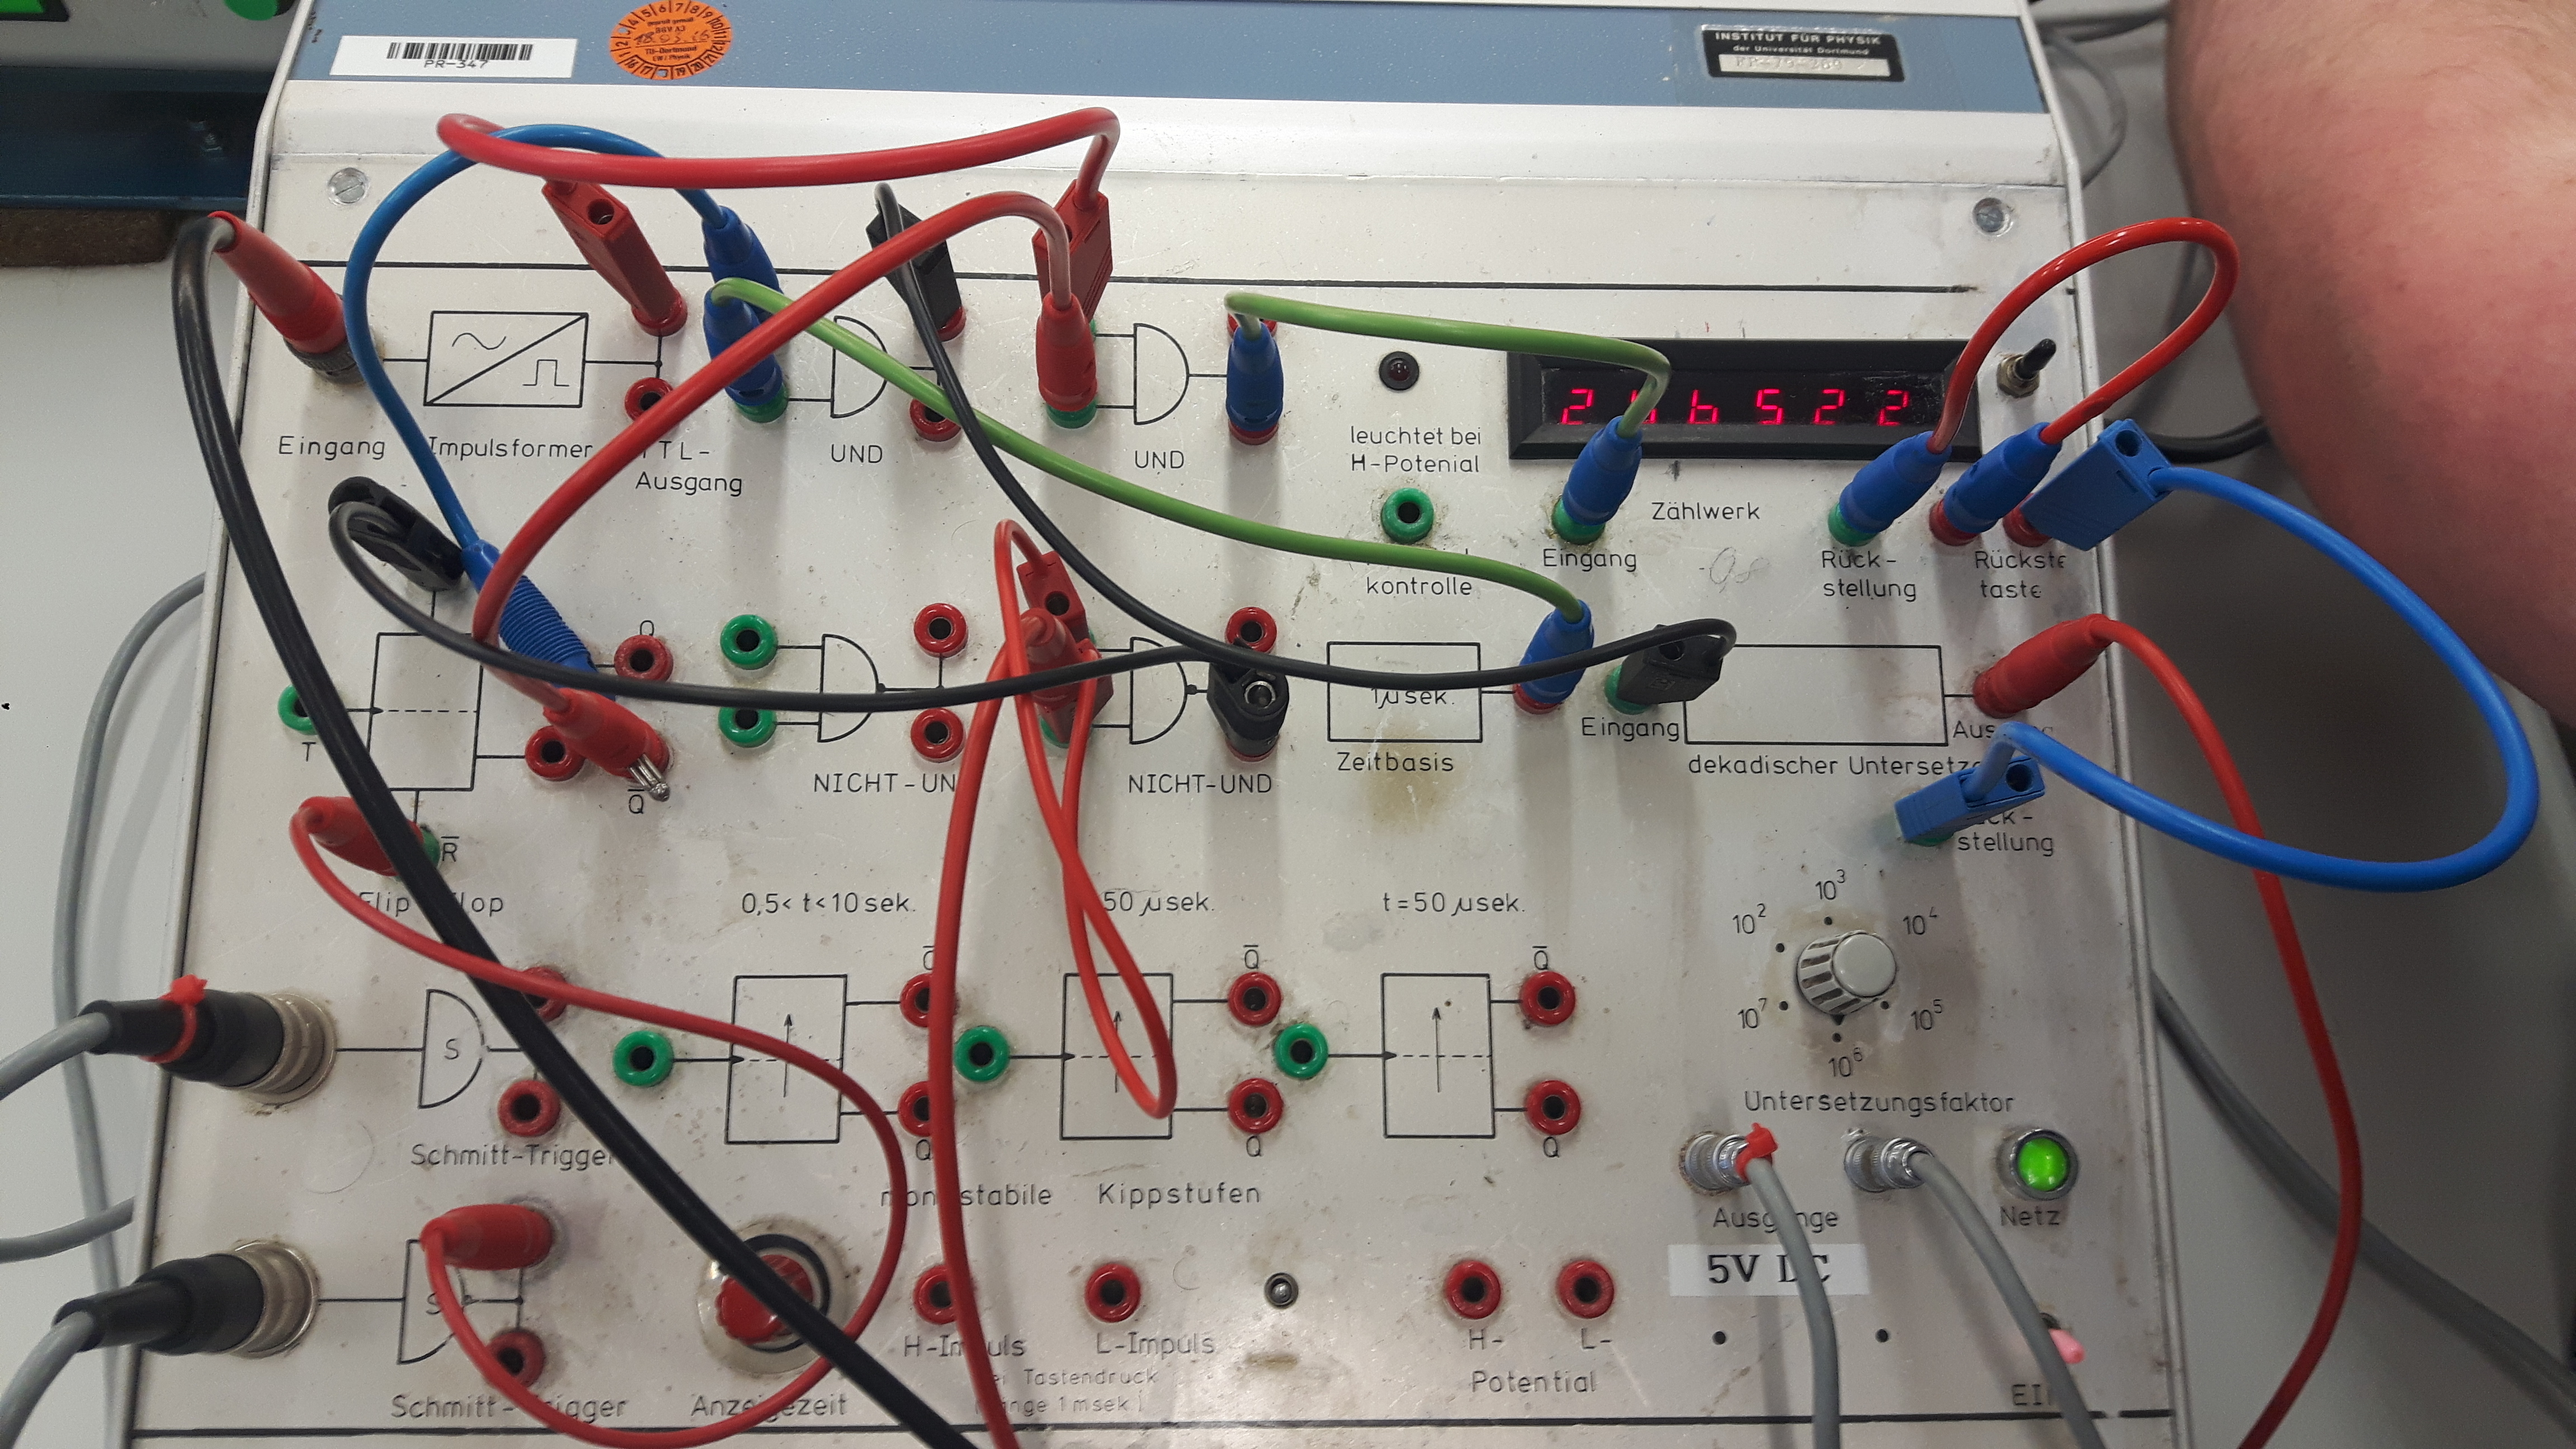
\includegraphics[width = \textwidth]{./Abbildungen/Frequenzmessung-Schranken.jpg}
  \caption{Schaltung zur Messung der geschwindigkeitsabhängigen Frequenz}
  \label{fig:vf-Schaltung}
\end{figure}

Zunächst wird die Ruhefrequenz $\nu_0$ gemessen. Hierzu wird der Lautsprecher
direkt vor dem Mikrophon aufgebaut und das Signal durch einen Verstärker in die
Schaltung \ref{fig:Ruhefrequenz} eingespeißt. Anschließend wir die Schaltung
\ref{fig:vf-Schaltung} verkabelt. Diese Schaltung zählt eine Sekunde lang
(nachdem die Lichtschranke unterbrochen wurde), wie viele Wellenberge am
Mikrophon ankommen. Des Weiteren wird der Lautsprecher auf den Wagen gestellt,
sodass er sich auf das Mikrophon zu bewegt (bzw. davon entfernt).
Der entsprechende Gesamtaufbau ist Abb. \ref{fig:vf} zu entnehmen.

\subsection{Schwebung}
\label{sec:Schwebung}
Bei dieser Variante der Bestimmung der Auswirkungen des Doppler-Effekts werden
Mikrophon und Lautsprecher direkt nebeneinander gestellt und ein
Schallreflektierender Schirm auf dem Wagen montiert. Auf diese Weise nimmt das
Mikrophon sowohl das reflektierte, als auch das vom Lautsprecher emmitierte
Signal direkt auf. Diese beiden Signale überlagern sich zu einer Schwebung,
aus welcher $\Delta \nu$ mit Hilfe eines Tiefpassfilters herausgefiltert werden kann.
Dieses gefilterte Signal wird dann in die Schaltung \ref{fig:vf-Schaltung}
gespeißt. Dieser Aufbau ist in Abb. \ref{fig:Schwebung} dargestellt.

\begin{figure}
  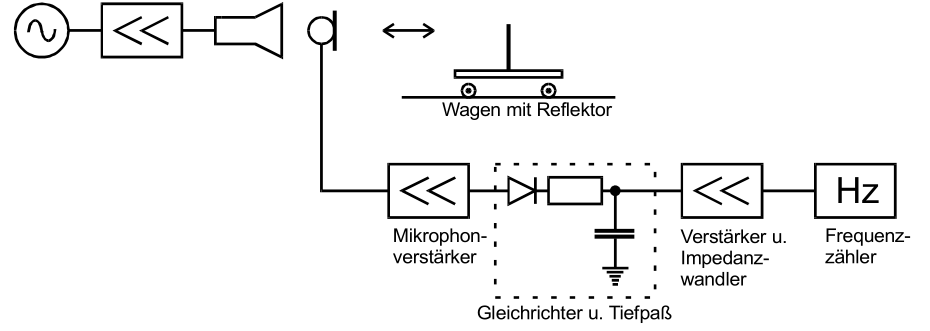
\includegraphics[width = \textwidth]{./Abbildungen/Schwebung.PNG}
  \caption{Aufbau zur Messung des Dopplereffekts mittels Schwebungsmethode \cite{Anleitung}.}
  \label{fig:Schwebung}
\end{figure}
